\chapter{Solution architecture}
\label{chap:evaluation-framework}

\section*{}

This chapter describes the proposed architecture for managing waste containers
fill status and calculating efficient routes. It starts by specifying, in
section~\ref{section:framework}, all the modules and the information workflow of
the framework. Section~\ref{section:languages} presents the technologies used to
implement each module, while section~\ref{section:formats} specifies the data
formats in which information is exchanged between modules.

Section~\ref{section:metrics} defines the metrics chosen to evaluate the
optimization algorithms, so that they may be quantified and properly compared.

Section~\ref{section:datasets} introduces the datasets used throughout this
study. Implemented algorithms will be applied to these datasets, and the
resulting routes will be evaluated using the metrics previously defined in
section~\ref{section:metrics}.

A subset of these datasets, defined in
section~\ref{section:validation-datasets}, will be used to validate the
algorithms' implementations. These datasets are widely used throughout the
literature to benchmark algorithms, and their optimal solutions has usually
already been determined.

Section~\ref{section:realistic-datasets} presents a
second subset of datasets, whose properties are similar to those of the datasets
obtained when the monitoring system is deployed. These will be used to compare
the algorithms' performance.




\section{Framework workflow}
\label{section:framework}

This project is structured in a modular way; this chapter enumerates and
describes each one of the modules, defining what is required and produced in
each step. 

To understand the following architecture and underlying information flow, one
must have in mind that this project has two major components. First, several
optimization algorithms must be compared, using both real and fabricated
scenarios. In second place, the system must be ready to be integrated with the
fill status monitoring solution being developed at \fhp{}.

First, the optimization module itself must receive a dataset describing the
collection scenario, which should contain:

\begin{itemize}
  \item city topology
  \item waste containers' location
  \item vehicle starting point
  \item minimum and maximum number of vehicles
\end{itemize}

With this information, it shall produce a single file describing one route per
used vehicle. This file can then be fed to the evaluation module, which
determines the solution's performance, according to several metrics, described
later on in section~\ref{section:metrics}. This performance evaluation
mechanism will be used mainly during the comparison phase of this project,
while the optimization module will be used in both phases.

Dataset information is gathered from several different places: map
retrieved from GIS sources, as described in
section~\ref{section:datasets}; containers' fill status can be stochastically
generated or obtained from the monitoring system's database. These data are
then normalized and merged to form a single dataset file. The full information
flow can be seen in figure~\ref{fig:architecture}.

\begin{figure}[H]
  \begin{center}
    \leavevmode
    %
\usetikzlibrary[positioning]
\usetikzlibrary{shapes.misc}
\tikzstyle{every entity} = [color=black,draw=black]

\begin{tikzpicture}[>=stealth']

\drawdatabase{osm}{-4cm}{-0.625cm}{OpenStreet Map}
\drawdatabase{sensordata}{-4cm}{-5cm}{Sensor Data}

\node[entity] (citygen) [above=of osm] {\parbox{2cm}{\begin{center}City random generator\end{center}}};
\node[entity] (retriever) [right=of sensordata] {Retriever};
\node[document] (citymap) [below=of citygen,above=of osm,right=of osm] {\parbox{0.5cm}{\begin{center}City map\end{center}}};
\node[entity] (containergen) [below=of citygen,right=of citymap] {\parbox{2cm}{\begin{center}Container random generator\end{center}}};
\node[document] (containerdata) [below=of containergen] {\parbox{1cm}{\begin{center}Container data\end{center}}};

\draw (citygen) edge [->] (citymap);
\draw (osm) edge [->] (citymap);
\draw (citymap) edge [->] (containergen);
\draw (sensordata) edge [->] (retriever);
\draw (retriever) edge [->] (containerdata);
\draw (containergen) edge [->] (containerdata);

\end{tikzpicture}

    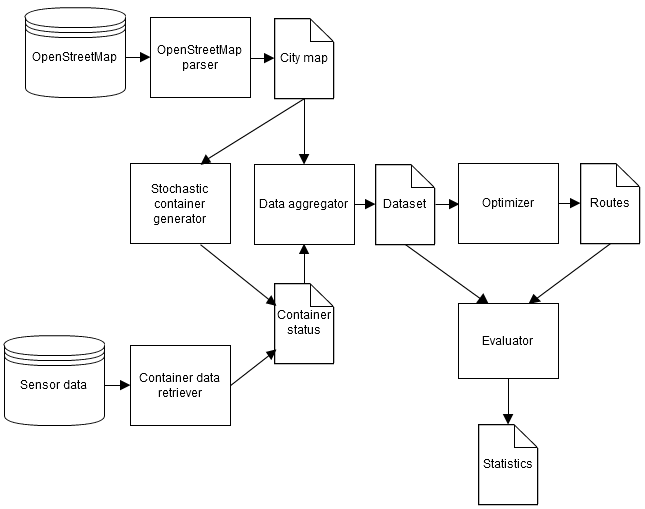
\includegraphics[width=1.0\textwidth]{architecture.png}
    \caption{Project architecture}
    \label{fig:architecture}
  \end{center}
\end{figure}

Note that there is the need to manage independent city and containers' status
files before creating a normalized dataset. This happens because the stochastic
container generator depends on the city file to create valid scenarios.

\section{Implementation details}
\label{section:languages}

To implement this framework, there was the need to decide which technologies to
use, regarding several modules.

Figure~\ref{fig:architecture} shows the necessity of a database management
system (DBMS), to maintain information about the containers' fill status. Due to
the simple nature of the information model stored in the database, the choice of
which DBMS to use is not critical. Additionally, the load of the DBMS will not
be too high, as the optimization process is only run once per day. With this in
mind, it was decided to use the MySQL DBMS, as it is both free and widely used
in high profile projects, such as the \textit{Wikimedia Foundation} and
\textit{Yahoo! Finance}~\citep{Balanescu2008}.

Modules such as the \textit{data aggregator}, \textit{OpenStreetMap parser},
\textit{Container data retriever} and \textit{Stochastic container generator}
were developed using a combination of C++ and bash scripting. C++ was used to
apply complex transformations to the data, which involved handling large files.
Bash scripting was used as an utility to invoke MySQL queries and convert the
retrieved data into a more convenient format.

All the algorithms in the optimization module were implemented in C++. As the
algorithm implementations need to be efficient (both regarding running time and
memory), the usage of interpreted languages, such as Ruby or Python, was
discarded. C++ was chosen due to the author's familiarity with the language,
thus accelerating the development phase.

The evaluation module was also implemented in C++, so that its code could be
shared with the optimization module.

\section{Data formats}
\label{section:formats}

As seen in figure~\ref{fig:architecture}, there are five different files that
carry information from one module to the next. To ease implementation, all five
formats were specified using the same notation.

Examples of common data interchange formats are XML (Extensible Markup
Language) and JSON (JavaScript Object Notation). Advantages of such standards
are, for example, the ready availability of several parsers for a great number
of languages~\citep{site:json,site:xml}, their openness and simplicity.

Between these two notations, it was decided to use the JSON format. It was
chosen because it is simpler than XML and because it was specifically designed
to be a lightweight computer data interchange format, whereas XML was designed
to be a document interchange format~\citep{site:json}.

JSON is based on two universal data structures: ordered lists and keyed lists
(from here on out called \textit{objects}). The latter structure is also known
in various programming languages as a \textit{dictionary}, \textit{hash table},
\textit{associative array} and others. There are also primitive types
available, such as strings, numbers and three constants: \texttt{true},
\texttt{false} and \texttt{null}.

While objects' keys must be strings, their values can be of any type, either
primitive or not. The same is true for ordered lists' elements. Further details
regarding JSON syntax can be found in the RFC 4627~\citep{site:rfc-json}.

The following sections in this chapter will describe each one of the five
formats present in this system's architecture.






\subsection{City map format}
\label{section:map-format}

To simulate the waste generation and collection, there is the need to provide a
topological city map. This topological map must be represented as a directed
weighted graph, so that routing algorithms may be applied. A city is usually a
sparse graph --- each vertex, representing a street intersection, has a reduced
number of arcs. This leads to the conclusion that a adjacency list
representation should be used.

A city map file is composed of a single JSON object
(\textbf{\texttt{city\_map}}). This contains two pairs of key/values; one of
them, whose key is \texttt{name}, has a string as its value and represents the
city map name, being used as human-readable metadata. Its second pair has the
key \texttt{graph} and its value represents the city topology, described as an
adjacency list --- a data structure commonly used to describe graphs.  This
adjacency list is defined as an ordered list, where each element represents a
vertex.

Each vertex is represented by a JSON object, containing a key/value pair for
its latitude (\texttt{lat}) and its longitude (\texttt{lon}), with both values
being represented as JSON numbers. A third key/value pair is present; its key
is \texttt{roads}, and its value defines the vertex's neighbors. This neighbor
list is encoded as a JSON ordered list, with each element identifying the
neighbor by its index in the main adjacency list.

A sample graph and its corresponding \textbf{\texttt{city\_map}} object can be
seen in figure~\ref{fig:city-map-example}.


\begin{figure}[th]
  \begin{center}
    \leavevmode
    \begin{tikzpicture}[>=stealth']
\SetVertexMath
\Vertex[x=0,y=0.0]{0}
\Vertex[x=2,y=-1]{1}
\Vertex[x=4,y=1.0]{2}
\Vertex[x=4,y=-1.0]{3}
\Vertex[x=2,y=1]{4}

\SetUpEdge[style=->]
\Edges(4,2,4)
\Edges(4,3,4)
%\Edge[style={<->,out=45,in=-45}](3)(f_0)
%\Edge[style={<->,out=-45,in=45}](2)(f_1)
\Edges(4,1,0,4)
\Edges(1,3,1)
\Edges(2,3,2)

\draw
  (4.75,2) --
  (-0.5,2) --
  (-0.5,-2) --
  (4.75,-2) --
  (4.75,2) --
  (14.5,2) --
  (14.5,-2) --
  (4.75,-2) --
  cycle;

\node[right=4.5cm] {
  \begin{minipage}{10cm}
  \begin{verbatim}
  {"name": "Sample city",
   "graph": [
    {"lat": 0, "lon": 0, "roads": [4]},
    {"lat": 2, "lon": -1, "roads": [0,3]},
    {"lat": 4, "lon": 1, "roads": [3,4]},
    {"lat": 4, "lon": -1, "roads": [1,2,4]},
    {"lat": 2, "lon": 1, "roads": [1,2,3]}
  ]}
\end{verbatim}
\end{minipage}
};

\end{tikzpicture}


    \caption{An example city topology map and its JSON equivalent.}
    \label{fig:city-map-example}
  \end{center}
\end{figure}



\subsection{Containers status format}
\label{section:container-format}

The containers' fill status file contains, for each container, its location ---
latitude and longitude --- and the current amount of waste stored in it. This
is represented by a JSON ordered list, with an element per container. Each
container element is a JSON object and contains three key/value pairs: one for
its latitude (\texttt{lat}), one for its longitude (\texttt{lon}) and one for
its current fill (\texttt{fill}). An example JSON object is available in
figure~\ref{fig:containers-example}.

\begin{figure}[th]
  \begin{center}
    \leavevmode
      \begin{minipage}{9cm}
    \begin{verbatim}
[
 {"lat": 0.0, "lon": 0.0, "fill": 43.01},
 {"lat": 4.1, "lon": -0.9, "fill": 18.47}
]
    \end{verbatim}
    \end{minipage}
    \caption{An example containers' fill status JSON file.}
    \label{fig:containers-example}
  \end{center}
\end{figure}





\subsection{Dataset format}
\label{section:dataset-format}

After obtaining both the city map file and the containers' status file, they
must be merged together to form a single dataset file. This action is performed
by the \textit{normalizer} module, shown previously in figure~\ref{fig:architecture}.

This format contains both features regarding the city topology and the
containers' fill status. Each container geographical position is matched
against the graph's vertices and its fill status information is added to the
closest vertex.

The dataset schema is similar to the one presented in
section~\ref{section:map-format}, with a few changes. First, for each vertex in
which a waste container is present, there is an additional key/value pair
representing its fill status, as defined in
section~\ref{section:container-format}. Second, two new key/value pairs must be
added to the main JSON object; one regarding the maximum number of trucks to
use (\texttt{max\_trucks}) and one regarding the starting/ending node
(\texttt{depot}). These two extra parameters must be defined when running the normalization process,
and are not present in any of the previous data file formats.

Taking the examples presented in the two previous sections, they could be
normalized into the dataset file present in figure~\ref{fig:dataset-example}.

\begin{figure}[th]
  \begin{center}
    \leavevmode
      \begin{minipage}{12cm}
    \begin{verbatim}
{"name": "Sample city",
 "max_trucks": 3,
 "depot": 1,
 "graph": [
  {"lat": 0, "lon": 0, "roads": [4], "fill": 43.01},
  {"lat": 2, "lon": -1, "roads": [0,3]},
  {"lat": 4, "lon": 1, "roads": [3,4]},
  {"lat": 4, "lon": -1, "roads": [1,2,4], 18.47},
  {"lat": 2, "lon": 1, "roads": [1,2,3]}
]}
    \end{verbatim}
    \end{minipage}
    \caption{Complete dataset example object, constructed from previous examples.}
    \label{fig:dataset-example}
  \end{center}
\end{figure}





\subsection{Routes format}
\label{section:routes-format}

The optimization module must process a single dataset file and determine a
near-optimal set of routes --- one for each vehicle. Each vehicle route can be
defined as an ordered list of references to the city vertices.

When dealing with commercial scenarios, each vertex there should be paired with
a boolean indicator that tells if the vehicle must empty the waste container
present at that location. In the Rollon-Rolloff scenario, this additional
flag indicates if the vehicle should load/unload a container at that location.

The set of routes can be defined as a JSON ordered list, with each element
defining a single route. Each route can also be represented by an ordered list
of vertex references. These are themselves defined as ordered lists of two
values; the first value represents the vertex index, while the second is a
boolean value, determining if the vehicle should or should not act on that
specific location.

Figure~\ref{fig:routes-example-rr} shows an example of a two-vehicle routes
file, in the Rollon-Rolloff scenario, after applying an optimization technique
to the previously shown dataset. Each vehicle starts by loading an empty
container at vertex 1, moves to a location with a full container and switches
the empty with the full one. Then, both vehicles proceed back to the depot
location, where they deposit the picked up containers.

\begin{figure}[th]
  \begin{center}
    \leavevmode
      \begin{minipage}{14cm}
    \begin{verbatim}
[
 [[1, true], [4, true], [4, true], [0, false], [1, true]],
 [[1, true], [3, true], [3, true], [1, true]]
]
    \end{verbatim}
    \end{minipage}
    \caption{Rollon-Rolloff set of routes example, representing two vehicles.}
    \label{fig:routes-example-rr}
  \end{center}
\end{figure}




\subsection{Statistics format}
\label{section:statistics-format}

The fifth data format regards the statistics obtained when evaluating the
routes obtained by a given optimization module. These metrics are calculated
based on the routes and the dataset files. The output object is represented as
a JSON object, where each key/value pair represents a different metric. This
representation is left open, as metrics may be added and/or removed during the
algorithm comparison phase.








\section{Evaluation metrics}
\label{section:metrics}

Performance evaluation of the implemented optimization framework requires the
definition of quantifiable metrics. As the goal is to reduce collection costs,
an important metric is the total number of kilometers that vehicles travel
during waste collection. The lower the number of kilometers is, the better.

Although the total distance is the main evaluation metric, there are additional
metrics that may be used to evaluate a solution. The average ratio between a
vehicle's capacity and the total urban waste it collects may be important to
evaluate collection efficiency.





\section{Datasets}
\label{section:datasets}

This section will present datasets used for algorithm validation. This will be
followed by the description of the methods used to obtain large datasets that
share the same properties as the ones to be used in production, when the
monitoring system is deployed.

\subsection{Validation datasets}
\label{section:validation-datasets}

Routing problems have been widely studied over the last decades; this has led
to the establishment of standard datasets for benchmarking algorithms and
implementations, one of them being the TSPLIB\cite{GerhardReinelt01011991}.
There are datasets for the \textit{Capacitated Vehicle Routing Problem}, both
\textit{Symmetric} and \textit{Asymmetric Traveling Salesman Problem} and other
related routing problems. ATSP instances have been solved optimally; as such,
they are accompanied by their respective optimum route cost.

This library can be used to validate the algorithm implementations described in
chapter~\ref{chap:algorithms}, as it allows one to measure the performance gap
between a given solution and the optimal route.

Table~\ref{tab:tsplib-atsp} shows the ATSP validation instances, including the
number of nodes and the optimum route cost, while table~\ref{tab:tsplib-cvrp}
shows the CVRP validation instances. In the latter case, an optimum route cost
is not available. This is due to the fact that these datasets can be used to
formulate several problems. For example, one might consider the number of
vehicles specified in the dataset as a fixed, minimum or maximum value. It
might also be possible to disregard the number of vehicles specified by the
dataset. As such, table~\ref{tab:tsplib-cvrp} only presents reference values
obtained when considering a fixed number of vehicles.

\begin{table}[H]
  \caption{Asymmetric Traveling Salesman Problem datasets, presenting the
  number of vertices and the optimum route cost.}
  \begin{center}
    \begin{tabular}{lll }
      \hline
      Name & Number of vertices & Optimum route cost \\
      \hline
      br17	  &  17 & 39    \\
      ftv33	  &  33 & 1286  \\
      ftv35	  &  35 & 1473  \\
      ftv38	  &  38 & 1530  \\
      p43	    &  43 & 5620  \\
      ftv44	  &  44 & 1613  \\
      ftv47	  &  47 & 1776  \\
      ry48p	  &  48 & 14422 \\
      ft53	  &  53 & 6905  \\
      ftv55	  &  55 & 1608  \\
      ftv64	  &  64 & 1839  \\
      ftv70	  &  70 & 1950  \\
      ft70	  &  70 & 38673 \\
      kro124p	& 124 & 36230 \\
      ftv170	& 170 & 2755  \\
      \hline
    \end{tabular}
  \end{center}
  \label{tab:tsplib-atsp}
\end{table}
\vfill

\begin{table}[H]
  \caption{Capacitated Vehicle Routing Problem datasets, presenting the
  number of vertices and a reference route cost.}
  \begin{center}
    \begin{tabular}{lll}
      \hline
      Name & Number of vertices & Reference route cost \\
      \hline
      eil13   &   13 &   247 \\
      eil22   &   22 &   375 \\
      eil23   &   23 &   569 \\
      eil30   &   30 &   534 \\
      eil31   &   31 &   379 \\
      eil33   &   33 &   835 \\
      eil51   &   51 &   521 \\
      eilA76  &   76 &   682 \\
      eilB76  &   76 &   735 \\
      eilC76  &   76 &   830 \\
      eilD76  &   76 &  1021 \\
      eilA101 &  101 &   815 \\
      eilB101 &  101 &  1071 \\
      gil262  &  262 &  6119 \\
      \hline
    \end{tabular}
  \end{center}
  \label{tab:tsplib-cvrp}
\end{table}



\newpage
\subsection{Realistic city datasets}
\label{section:realistic-datasets}

In order to properly evaluate the developed algorithms, there was the need to
obtain realistic datasets that represented the street topology of real cities.
These datasets must be similar to those to be obtained by the monitoring
system, so that results are as reliable as possible.


\subsubsection{\osm{}}
\label{section:osm}

To obtain realistic city maps, a tool to extract and convert topological maps
from \textit{OpenStreetMap.org} was developed. \textit{OpenStreetMap.org} is an
collaborative and open source initiative which aims to create a free editable
map of the world~\cite{Mordechai2008}. Users may add information by editing the
world map manually --- using the web editor --- or by submitting data from GPS
devices.

Figure~\ref{fig:porto} shows the topological map of the city of Porto,
Portugal, which was imported from \textit{\osm}. Unfortunately, both the
connectivity and the structure of the city of Porto are highly inaccurate. This
leads to a strongly disconnected graph, in which several adjacent streets are
not connected. This happens for several reasons. First, some of the information
of the streets direction is outdated. Second, users contributing to this
project may have had little attention to detail regarding the graph
connectivity, aiming only to add visual information of the city streets. Users
may also have been deprived of the necessary tools to provide accurate
information regarding street connectivity.

\begin{figure}[th]
  \begin{center}
    \leavevmode
    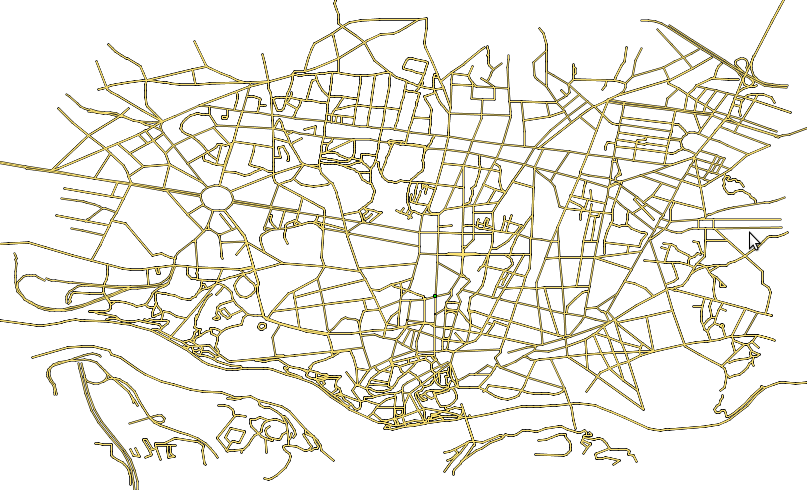
\includegraphics[width=0.75\textwidth]{porto}
    \caption{The city of Porto, Portugal, retrieved from \osm{} and loaded onto the current framework viewer.}
    \label{fig:porto}
  \end{center}
\end{figure}

\subsubsection{Waste generation}
\label{section:waste-generation}

Having no current access to real waste containers location and fill status ---
as the monitoring platform is not yet deployed --- there was the need to
generate this information artificially, using a stochastic approach. Waste
containers were scattered in street intersections following different patterns
according to the following process:

The algorithm starts by selecting $k$ road intersections (represented by a
graph vertex) on the city map as cluster centers. A number $d_i$ in the range
$[0, 1]$ is assigned to each cluster, representing the cluster's waste
container density. Then, until all intersections belong to a cluster, $k$
vertices are chosen arbitrarily from each of the clusters' neighborhood and
added to the respective cluster. When a vertex is added to a cluster it is
decided, with probability $d_i$, if it should contain a full waste container.

\subsubsection{Generated datasets}
\label{section:large-datasets}

This approach was applied to three different city topological maps --- Leeds,
Lisbon and London --- using different clustering parameter configurations. This
yielded fifteen large datasets, whose number of vertices ranges from $518$ to
$7628$. Table~\ref{tab:large-datasets} shows information about these datasets
--- both the number of nodes and the cities in which their topology was based.

\begin{table}[h!]
  \caption{Large realistic Capacitated Vehicle Routing Problem datasets}
  \begin{center}
    \begin{tabular}{lll}
      \hline
      Name & Number of vertices & City \\
      \hline
      hp518 & 518 & Leeds \\
      hp841 & 841 & Leeds \\
      hp904 & 904 & Leeds \\
      hp1287 & 1287 & Leeds \\

      hp1175 & 1175 & London \\
      hp1849 & 1849 & London \\
      hp2038 & 2038 & London \\
      hp2206 & 2206 & London \\

      hp2561 & 2561 & Lisbon \\
      hp3481 & 3481 & Lisbon \\
      hp3859 & 3859 & Lisbon \\
      hp4109 & 4109 & Lisbon \\
      hp4628 & 4628 & Lisbon \\
      hp6247 & 6247 & Lisbon \\
      hp7628 & 7628 & Lisbon \\
      \hline
    \end{tabular}
  \end{center}
  \label{tab:large-datasets}
\end{table}

\section{Chapter summary}
\label{section:implementation-summary}

This chapter presented the design for the fill status monitoring framework ---
the information workflow, data interchange formats and the technologies have
been specified. Additionally, sections~\ref{section:metrics}
and~\ref{section:datasets} specified the metrics and datasets with which to
validate the waste collection route optimization approaches.

The following chapter will introduce the optimization algorithms used throughout
this study.

